\documentclass{standalone}

\usepackage{tikz}
\usetikzlibrary{calc}

\begin{document}

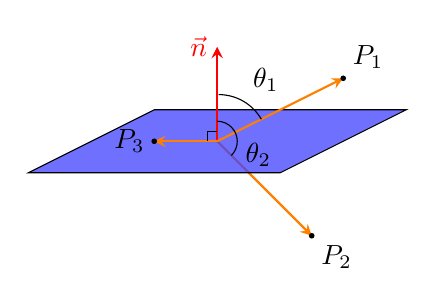
\begin{tikzpicture}[scale=0.8]

\coordinate (O)  at (0,0);
\coordinate (P1) at (-3,-0.5);
\coordinate (P2) at ($(P1)+(2,1)$);
\coordinate (P3) at ($(P2)+(4,0)$);
\coordinate (P4) at ($(P3)+(-2,-1)$);
\coordinate (N1) at (0,0);
\coordinate (N2) at ($(N1)+(0,1.5)$);
\coordinate (Q1) at (2,1);
\coordinate (Q2) at (1.5,-1.5);
\coordinate (Q3) at ($(N1)+(-1,0)$);

\draw[-stealth, thick, orange] (N1)--(Q2);
\filldraw[black, fill=blue!75!white, fill opacity=0.75] (P1)--(P2)--(P3)--(P4)--cycle;
\draw[-stealth, red, thick] (N1)--(N2) node[left] {$\vec n$};

\draw[-stealth, thick, orange] (N1)--(Q1);
\draw[-stealth, thick, orange] (N1)--(Q3);

\draw ($(N1)+0.35*(Q1)$) arc (30:90:0.7826) node[midway, above right] {$\theta_1$};
\draw ($(N1)+0.15*(Q2)$) arc (-45:90:0.3182) node[midway,below right] {$\theta_2$};
\draw ($(N1)+(0,0.15)$)--++(-0.15,0)--++(0,-0.15);

\draw[fill=black] (Q1) circle (1pt) node[above right] {$P_1$};
\draw[fill=black] (Q2) circle (1pt) node[below right] {$P_2$};
\draw[fill=black] (Q3) circle (1pt) node[left] {$P_3$};

\end{tikzpicture}

\end{document}